\documentclass[12pt]{bsc}

\usepackage[T1,MeX]{polski}
\usepackage[utf8]{inputenc}
\usepackage[T1]{fontenc}
\usepackage{txfonts}

\usepackage[polish]{babel}
\usepackage{graphicx}
\usepackage{fancyvrb}
\usepackage{pdfpages}

\usepackage{enumitem}%
\usepackage{listings}
\usepackage[pdftex,pdfstartview=FitH,unicode]{hyperref}
\usepackage[justification=centering]{caption}

\graphicspath{{./img/}}
% ********* citing papers *********
\selecthyphenation{polish}




% ********* Colours for source code *********
%New colors defined below
\definecolor{codegreen}{rgb}{0,0.6,0}
\definecolor{codegray}{rgb}{0.5,0.5,0.5}
\definecolor{codepurple}{rgb}{0.58,0,0.82}
\definecolor{backcolour}{rgb}{0.95,0.95,0.92}%

%Code listing style named "mystyle"
\lstdefinestyle{mystyle}{
  backgroundcolor=\color{backcolour},
  commentstyle=\color{codegreen},
  keywordstyle=\color{magenta},
  numberstyle=\tiny\color{codegray},
  stringstyle=\color{codepurple},
  basicstyle=\ttfamily\footnotesize,
  breakatwhitespace=false,         
  breaklines=true,                 
  captionpos=b,                    
  keepspaces=true,                 
  numbers=left,                    
  numbersep=5pt,                  
  showspaces=false,                
  showstringspaces=false,
  showtabs=false,                  
  tabsize=2
}
\lstset{style=mystyle}

% ********* documents meta data **********
\makeatletter

\def\@title{Symulator sterownika do RET-a implementujący protokół AISG 2.0}
\def\@engTitle{Ret driver simulator for AISG 2.0 Device}
\def\@author{Paweł Koryciński}
\def\@promoter{dr Grzegorz Debita}
\def\@when{2020-02-15}
\def\@year{2020}
\def\@album{6749}

\makeatother

\begin{document}
  \renewcommand{\partname}{} % for the empty part title
  \renewcommand{\thepart}{} % for the empty part title
  

  \thispagestyle{empty}

\makeatletter

\begin{titlepage}
  \sffamily\bfseries
  
  \center{
    \fontsize{18}{18}\selectfont{
      WYŻSZA SZKOŁA INFORMATYKI I ZARZĄDZANIA
      ,,Copernicus'' we Wrocławiu
    }
    \rule[10pt]{\textwidth}{1pt}
    \raisebox{12pt}[0px]{
      \fontsize{16}{16}\selectfont\textmd{WYDZIAŁ INFORMATYKI}
    }
  }
  
  \flushleft\fontsize{14}{14}\selectfont{
    {\textmd{Kierunek studiów:}}
    Informatyka

    {\textmd{Poziom studiów:}}
    Studia pierwszego stopnia-inżynierskie
    
    {\textmd{Specjalność:}}
    Systemy i sieci komputerowe
  }
  
  \vspace*{40pt}
  \center{
    \fontsize{14}{14}\selectfont{PRACA DYPLOMOWA INŻYNIERSKA}
    
    \vspace*{30pt}
    \fontsize{14}{14}\selectfont\@author
    
    \vspace*{15pt}
    \fontsize{20}{20}\selectfont\@title
    
    \vspace*{20pt}
    \fontsize{14}{14}\selectfont\@engTitle
  }

  \vspace*{80pt}
  \flushright{  
    \fontsize{14}{14}\selectfont{Ocena pracy:}
    \makebox[220pt][r]{\fontsize{10}{10}\selectfont\dotfill}
    
    \fontsize{10}{10}\selectfont\textmd{(ocena pracy dyplomowej, data, podpis promotora) }
    
    \vspace*{50pt}
    \makebox[220pt][r]{\fontsize{10}{10}\selectfont\dotfill}
    
    \raisebox{4pt}{\fontsize{10}{10}\selectfont\textmd{(pieczątka uczelni)}}
  }
    
  \flushleft\fontsize{14}{14}\selectfont{
    Promotor:
    
    \bigskip\@promoter
  }

  \vspace*{20pt}
  \center{
    \rule[3pt]{\textwidth}{1pt}
    \fontsize{16}{16}\selectfont\textmd{WROCŁAW \@year}
  }
\end{titlepage}

\makeatother

\clearpage


  \tableofcontents
  \chapter*{Wykaz skrótów i symboli}
\addcontentsline{toc}{chapter}{Wykaz skrótów i symboli}
\noindent
\textbf{3GPP} --- organizacja normalizująca rozwój telefonii komórkowej;\newline
\textbf{5G} --- standard sieci komórkowej, następca LTE;\newline
\textbf{AISG 2.0} --- protokół bazujący na komunikacji half duplex oraz protokole HDLC;\newline
\textbf{Back-end} --- warstwa oprogramowania obsługująca niskopoziomową logikę biznesową;\newline
\textbf{bajt} --- najmniejsza adresowalna jednostka informacji pamięci komputerowej;\newline
\textbf{bit} --- najmniejsza jednostka informacji w odniesieciu do sprzętu komputerowej;\newline
\textbf{broadcast} --- rozgłoszeniowy tryb transmisji danych;\newline
\textbf{C++} --- język programowania;\newline
\textbf{CRC} --- Cyclic Redundancy Check - system sum kontrolnych;\newline
\textbf{CRC-16} --- 16-bitowy cykliczny kod nadmiarowy;\newline
\textbf{DB} --- database - baza danych;\newline
\textbf{debugowanie} --- proces analizy programu pod kątem zaistniałych błędów;\newline
\textbf{Debug} --- priorytet logowania wskazujący informacje potrzebne podczas debugowania;\newline
\textbf{delete} --- słowo kluczowe języka C++, którego użycie wywołuje destruktor obiektu;\newline
\textbf{driver} --- sterownik - program obsługujący urządzenie podłączone do komputera;\newline
\textbf{enkapsulacja} --- opakowanie danych z wyższej warstwy w warstwie niższej;\newline
\textbf{execute} --- metoda interfejsu klasy ICommand służąca do uruchomienia komendy;\newline
\textbf{Error} --- priorytet logowania informujący o błędnym wykonaniu programu;\newline
\textbf{Front-end} --- warstwa oprogramowania obsługująca odbiór danych od użytkownika;\newline
\textbf{gniazdo} --- dwukierunkowy punkt końcowy połączenia sieciowego;\newline
\textbf{GSM} --- Global System for Mobile Communications - standard telefonii komórkowej;\newline
\textbf{half duplex} --- połączenie w którym naprzemienne jest przesyłanie i odbieranie informacji;\newline
\textbf{HDLC} --- High-Data Link Control - protokół warstwy łącza danych;\newline
\textbf{HDLC body} --- ramka HDLC bez bajtów startu, stopu oraz sumy CRC;\newline
\textbf{h} --- hour - godzina;\newline
\textbf{Info} --- priorytet logowania informujący o ważnych etapach w wykonaniu programu;\newline
\textbf{klasa finalna} --- klasa po której nie można zdefiniować dziedziczenia;\newline
\textbf{little endian} --- cienkokońcowość;\newline
\textbf{LTE} --- Long Term Evolution - standard bezprzewodowego przesyłu danych;\newline
\textbf{ADDR} --- Address - adres docelowy urządzenia budujący ramkę;\newline
\textbf{CTRL} --- Control - bajt kontrolny ramki;\newline
\textbf{GI} --- Group Identifier - identyfikator grupy ramki;\newline
\textbf{GL} --- Group Length - długość groupy;\newline
\textbf{PI} --- Parameter Identifier - identyfikator parametru ramki;\newline
\textbf{PL} --- Parameter Length - długość wartości parametru ramki;\newline
\textbf{PL} --- Parameter Length - długość wartości parametru ramki;\newline
\textbf{PV} --- Parameter Value - wartość parametru ramki;\newline

\newpage
\chapter*{Wykaz skrótów i symboli}
\noindent
\textbf{metoda} --- funkcja należąca do klasy;\newline
\textbf{min} --- minute - minuta;\newline
\textbf{model OSI} --- model odniesienia łączenia systemów otwartych;\newline
\textbf{ms} --- milisecond - milisekunda;\newline
\textbf{N(R)} --- receive sequence number, numer porządkowy odebranej ramki;\newline
\textbf{N(S)} --- send sequence number, numer porządkowy wysłanej ramki;\newline
\textbf{null} --- wartość przypisywana do wskaźnika równa 0;\newline
\textbf{numer portu} --- jeden z parametrów gniazda, identyfikujący proces nim zarządzający;\newline
\textbf{OFDMA} --- metoda zwielokrotnienia w dziedzinie częstotliwości;\newline
\textbf{P/F bit} --- Pool/Final bit - obliczany podczas kalkulacji bajtu kontrolnego;\newline
\textbf{payload} --- fragment wiadomości zawierający jedynie istotne informacje;\newline
\textbf{POSIX Regexp} --- standard zapisu wyrażeń regularnych;\newline
\textbf{RAII} --- Resource acquisition is initialization - inicjowanie przy pozyskaniu zasobu;\newline
\textbf{ramka} --- pakiet danych;\newline
\textbf{RET} --- Remote Electrical Tilt - urządzenie zmieniające elektryczny kąt wiązki anteny;\newline
\textbf{RS-485} --- standard transmisji szeregowej;\newline
\textbf{std::any} --- klasa reprezentująca dowolny typ danych;\newline
\textbf{std::string} --- klasa reprezentująca łańcuch znaków;\newline
\textbf{std::vector} --- klasa reprezentująca danymiczną tablicę;\newline
\textbf{STL} --- Standard Template Library - biblioteka C++ w przestrzeni nazw std::;\newline
\textbf{s} --- second - sekunda;\newline
\textbf{Trace} --- priorytet logowania najniższej rangi;\newline
\textbf{UI} --- User Interface - interfejs użytkownika;\newline
\textbf{UMTS} --- Universal Mobile Telecommunications System - standard telefonii komórkowej;\newline
\textbf{UniqueId} --- złożenie numeru seryjnego wraz z kodem producenta;\newline
\textbf{USB} --- Universal Serial Bus - uniwersalna magistrala szeregowa;\newline
\textbf{Warning} --- priorytet logowania informujący o wykonaniu mogącym powodować błędy;\newline
\textbf{WCDMA} --- technika związana z dostępem do sieci radiowej;\newline

  \tableofcontents

\chapter{Wstęp}
\section{Wprowadzenie}
	Stacja nadawcza to zintegrowany system składający się z modułu systemowego, modułu rozszerzeniowego, radia oraz fizycznej anteny. 
	Ma ona na celu dostarczenie jak największej liczbie ludzi sygnału telekomunikacyjnego w celu nawiązania połączenia głosowego, 
	wysłania wiadomości tekstowej czy skorzystania ze skrzynki mailowej. Sęk w tym, że stacja nadawcza może być umieszczona w jednym miejscu, 
	natomiast odbiorcy, mogą przemieszczać się, co niesie ze sobą problem efektywnego pokrycia obszaru zasięgiem sieci operatora.
	W celu modyfikacji charakterystyki sygnału, anteny dipolowe usprawniane są o dodatkowe urządzenie o nazwie RET, które jest szeroko stosowane w technologiach GSM, WCDMA czy LTE.

\section{Cel pracy}
	Jako cel obrałem zaznajomienie się z protokołem komunikacyjnym AISG 2.0, którego użycie możemy zaobserwować na drodze pomiędzy 
	radio modułem a wzmacniaczem antenowym czy RET-em. 
	Jest to krok obowiązkowy przed rozpoczęciem zapoznawania się z AISG 3.0.
	Implementacja protokołu będzie wymagała wysokich umiejętności programowania w języku C++, 
	tworzenia testów, wdrażania wzorców projektowych oraz wiedzy z zakresu systemu kontroli wersji czy inżynierii oprogramowania.

\section{Motywacja}
	W przyszłości podłączenie RET-a do komputera (pomijając radio moduł) przy pomocy adaptera RS-232 -> USB, w celu skrócenia czasu testowania urządzenia.

  \include{zakres_bazaDanych_backEnd}
  % \chapter{Wstęp} masterPage
% \section{Zakres}


  \part{Część Przeglądowa}
  \chapter{RET}
	\section{Prezentacja urządzenia}
		Z angielskiego Remote Electrical Tilt, czyli urządzenie służące do zdalnej modyfikacji kąta głównej wiązki anteny, zwanego elektrycznym tiltem.
		\autocite{KATHREIN_RET_1}
		\begin{figure}[h!]
		\centering
		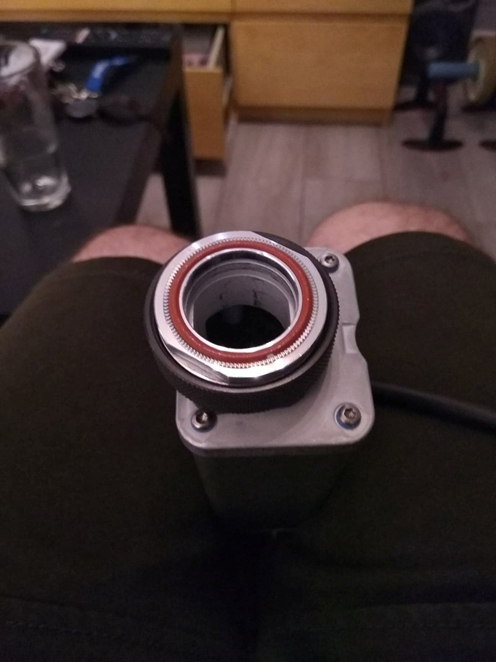
\includegraphics[scale=0.4]{Obrazki/RET_1.png}
		\caption{RetSimulator- Miejsce na antenę}
		\end{figure}

		\begin{figure}[h!]
		\centering
		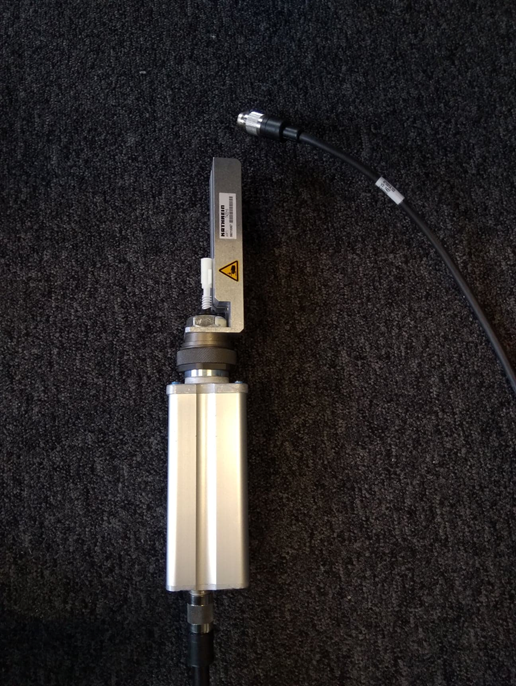
\includegraphics[scale=0.4]{Obrazki/RET_2.png}
		\caption{RetSimulator podłączonym kablem RS-485 oraz włożoną atrapą anteny}
		\end{figure}

	\section{Zmiana szerokości głównej wiązki fali elektromagnetycznej}
		\begin{figure}[h!]
		\centering
		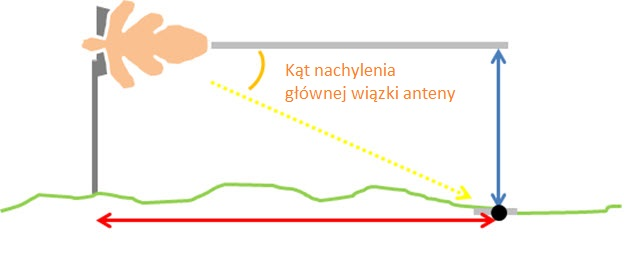
\includegraphics[scale=1.0]{Obrazki/Angle.jpeg}
		\caption{Rysunek przedstawiający kąt modyfikowany przy pomocy RET-a}
		\end{figure}
		
		Poniższe rysunki wygenerowano dzięki programowi Radio Mobile \autocite{RADIO_MOBILE_PAGE_1}
		Przedstawiono na nich szerokość wiązki promieni sygnału radiowego w osi poziomej \autocite{BEAMWIDTH_1}
		zmieniającą się dzięki modyfikacji elektrycznego kąta na wartość 40-tu stopni.
		Podczas symulacji użyto antenę Yagi, która aktualnie nie jest stosowana w technologii mobilnej z racji wspieranych
		przez nią częstotliwości, gdyż są one znacznie niższe aniżeli te wymagane przez WCDMA, LTE czy 5G, 
		aczkolwiek bardzo dobrze odzwierciedla działanie tych rzeczywistych ze względu na swoją charakterystykę kierunkową.
		\newline
		Antenę umieszczono przy WSIZ Copernicus. \newline
		Pomarańczowym kolorem widać tzw. kwiatek sygnału, który w przypadku kąta 0 stopni jest wydłużony oraz węższy,
		co pozwala pokryć śladowym zasięgiem nawet dalekie obszary, lecz do terenów bliżej zlokolizowanych dostarczony
		jest słabszy sygnał względem tego, który można otrzymać, zmieniając elektryczny kąt anteny na 40 stopni.
		Dzięki RET-owi, można skoncentrować wiązkę na mniejszym obszarze, oferując znacznie wyższe prędkości transmisji danych.

		\begin{figure}[h!]
		\centering
		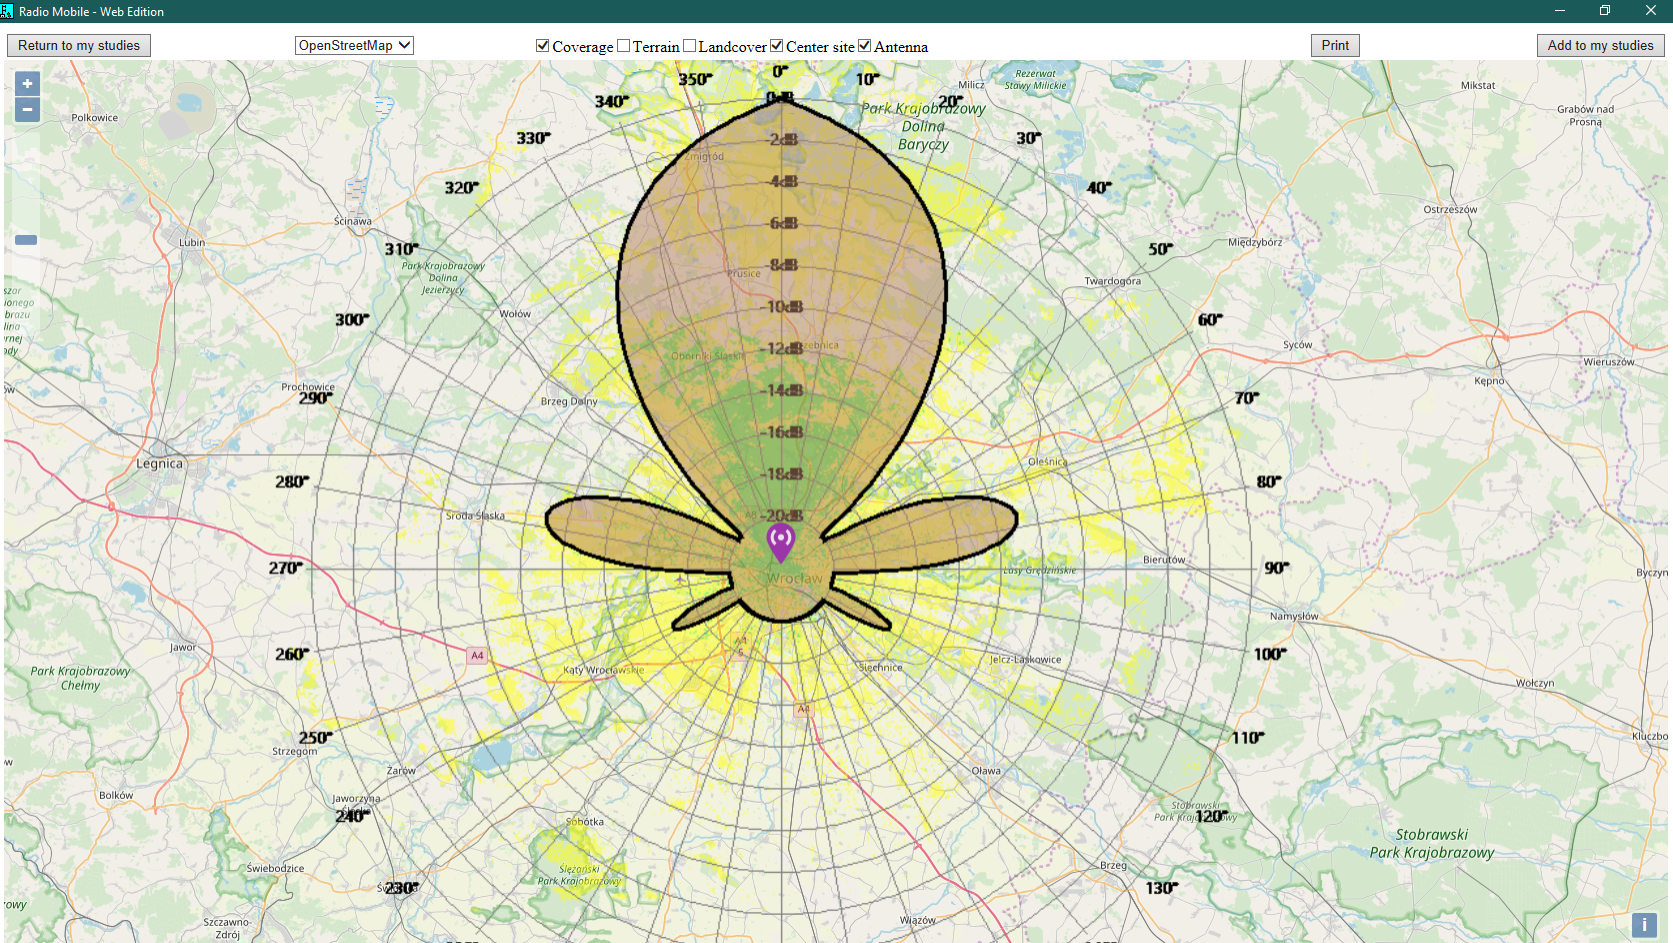
\includegraphics[scale=0.5]{Obrazki/Antenna_Yagi_Angle_0.png}
		\caption{Pokrycie obszaru sygnałem radiowym dzięki antenie Yagi, kąt elektryczny 0 stopni}
		\end{figure}

		\begin{figure}[h!]
		\centering
		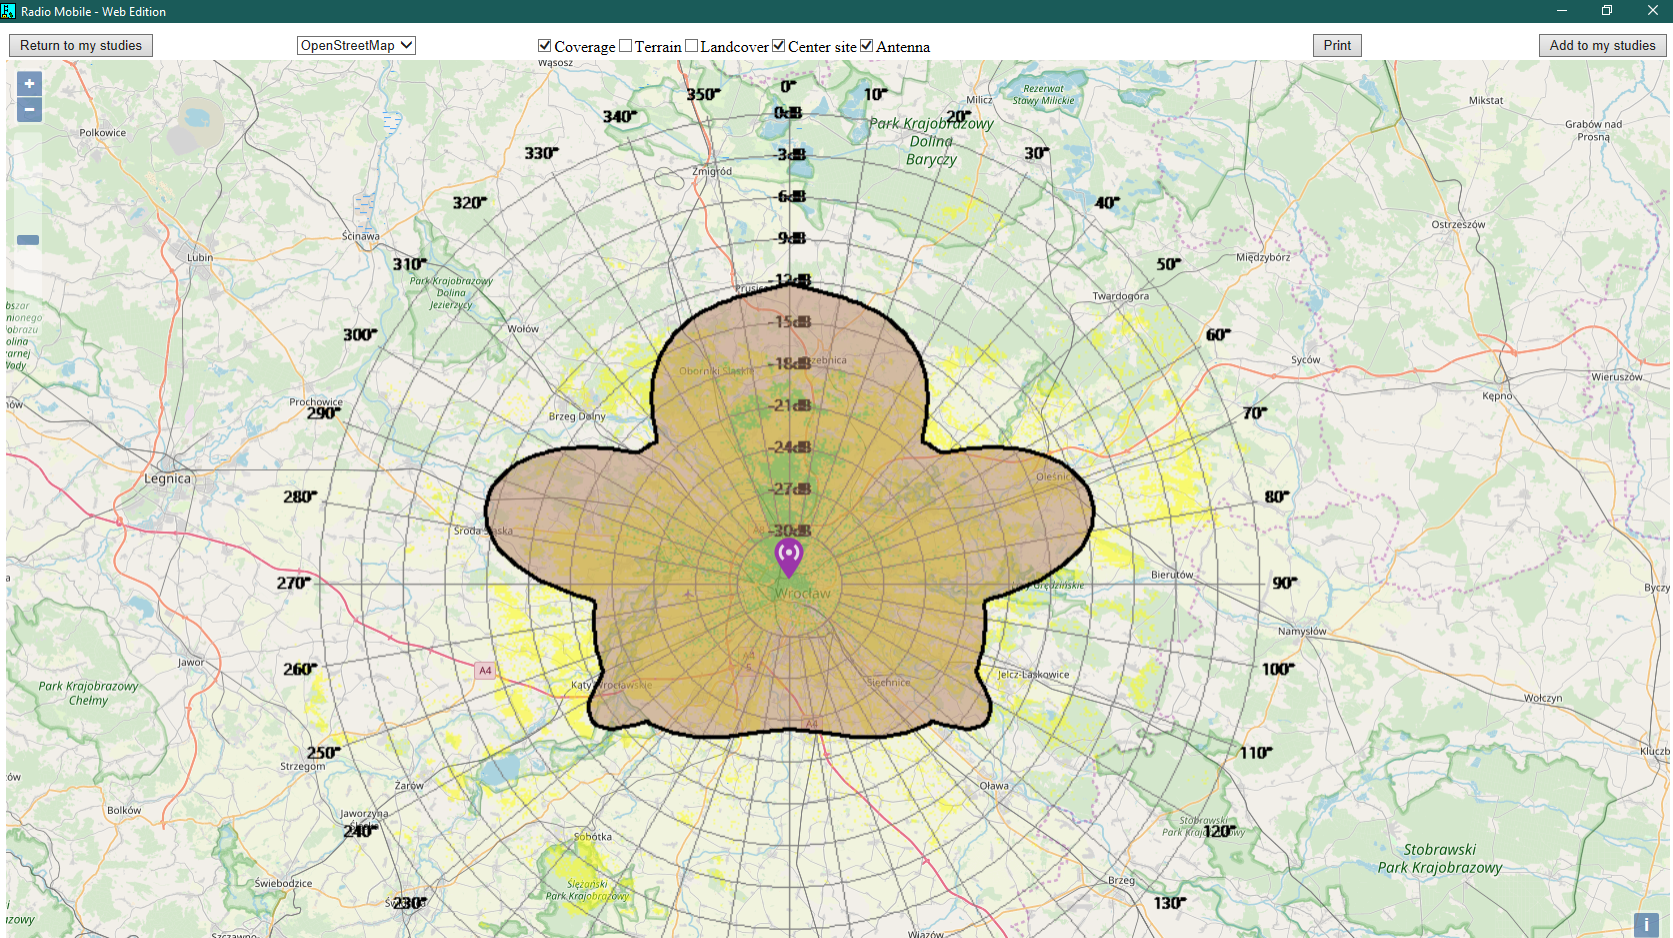
\includegraphics[scale=0.5]{Obrazki/Antenna_Yagi_Angle_40.png}
		\caption{Pokrycie obszaru sygnałem radiowym dzięki antenie Yagi, kąt elektryczny 40 stopni}
		\end{figure}

  \chapter{Protokół AISG 2.0}
	Symulator sterownika ma za zadanie odebrać od użytkownika polecenie w postaci komendy wieloargumentowej, 
	która zawierała będzie nazwę procedury rozpoznawanej przez odpowiednie warstwy protokołu komunikacyjnego \textit{AISG v2.0}
	realizującego podzbiór \textit{modelu OSI}.
	
	\section{Warstwy}
		\subsection{1-sza - Fizyczna}
		Realizacja projektu w kierunku emulacji fizycznego połączenia do urządzenia niesie ze sobą pewne zmiany na tej warstawie.\newline
		Należy pominąć obszar mechaniczny i elektryczny, a skupić się na obszarze funkcjonalnym oraz proceduralnym.
		\subsection{2-ga - Łącza danych}
		Rolą tej warstwy jest:
		\begin{itemize}
			\item Enkapsulacja[BIB] ramki \textit{HDLC Body} do ramki HDLC[BIB]
			\begin{itemize}
				\item Dodanie \textit{bitów} startu i stopu;
				\item Obliczenie oraz walidacja sumy CRC[BIB]
			\end{itemize}
			\item Budowa ramki typu XID podczas procedur negocjacji:
			\begin{itemize}
				\item Rozmiaru ramki;
				\item Unikalnego identyfikatora urządzenia, na które składa się numer seryjny oraz kod producenta;
				\item Wersji \textit{3GPP} oraz AISG urządzenia podrzędnego;
				\item Adresu;
			\end{itemize}
			\item Budowa ramki typu U w celu ustanowienia normalnego trybu komunikacji;
		\end{itemize}
		\subsection{7-ma - Aplikacji}
			\begin{itemize}
				\item Budowa ramki typu I;
				\item Rozpoznawanie wysokopoziomowej komendy kalibruj;
			\end{itemize}
  \section{HDLC}
Z języka angielskiego High-Level Data Link Control. Protokół warstwy łącza danych modelu OSI. 
Standard HDLC opisuje norma ISO, lecz szeroko stosuje się także implementację CISCO.
HDLC jest stosowany w technologii WAN, ponieważ obsługuje zarówno połączenia dwupunktowe, jak i wielopunktowe. 
Jest protokołem o orientacji bitowej oraz jest przezroczysty informacyjnie.\cite{WIKI_HDLC}
W przypadku, jeśli przesyłana wartość jest wielobajtowa, zastosowane jest podejście \textit{little endian}.
Głównym powodem, dla którego protokół utworzony w roku 1979 roku wciąż znajduje zastosowanie jest fakt, że jego implementacja pozwala w maksymalnym stopniu
wyeliminować możliwość utraty przesyłanej informacji dzięki mechanizmowi walidacji sumy \textit{CRC} oraz algorytmowi ewaluacji \textit{bajtu} kontrolnego. Dzięki temu urządzenie nadrzędne może nawet żądać
ponownego przesłania wcześniej otrzymanej wiadomości.
\subsection{Struktura ramki}
\begin{enumerate}
    \item Flaga startu - 0x7E;
    \item Adres stacji docelowej;
    \item Sterowanie - określa typ ramki oraz jej parametry w zależności od typu;
    \item Dane;
    \item Suma kontrolna FCS ( dwubajtowa ) - na przykład CRC-16;
    \item Flaga stopu - 0x7E;
\end{enumerate}
\subsection{Typy ramek}
\begin{itemize}
    \item Ramka I - Informacyjna;
    \item Ramka U - Nienumerowana;
    \item Ramka S - Nadzorująca;
    \item Ramka XID - Identyfikująca urządzenia;
\end{itemize}

  \section{Typy ramek HDLC}
	\subsection{Ramka XID}
	Jej nazwa pochodzi z języka angielskiego ,,exchange identification''. 
	Służy do przekazania urządzeniu podrzędnemu wiedzy na temat możliwości oraz charakterystyki komunikacji na warstwie łącza danych.\autocite{WIKI_ENG_HDLC}
	Odpowiadając na tego typu wiadomości, urządzenie podrzędne najczęściej zwraca tę samą wartość w przypadku zgodności 
	bądź najwyższą wspieraną, jeśli żądana jest zbyt duża. Szereg wysłanych i odebranych wiadomości XID nazywamy XID negocjacją.
	Tej ramki używamy również podczas ustalania prędkości komunikacji co jest częścią zestawiania warstwy fizycznej.
	Bajt kontrolny dla wiadomości przesyłanej będzie miał zawsze wartość 0xBF. \newline
	Bajty budujące ramkę:
	\begin{itemize}
		\item Adresu;
		\item Kontrolny;
		\item Identyfikujący format;
		\item Identyfikujący grupę;
		\item Długości grupy;
		\item Parametrów HDLC:
		\begin{itemize}
			\item Identyfikujący parameter;
			\item Długości parameteru;
			\item Wartości parametru;
		\end{itemize}
	\end{itemize} 
	Nie przez przypadek wspomniałem o parametrach HDLC zamiast o parametrze, gdyż równie dobrze można wysłać
    trzy wiadomości zawierające po jednym parametrze, jak i połączyć je w jedną większą.
	
  % \chapter{Protokół AISG 2.0}
\subsection{Ramka U}
Jej nazwa pochodzi z języka angielskiego ,,Unnumbered'' co oznacza nienumerowana.\autocite{WIKI_ENG_HDLC}
Wzięło się to z tego, że wielokrotnie wysłana wiadomość tego typu, zawsze posiada tą samą wartość bajtu kontrolnego.
Służy ona do zarządzania warstwą łącza danych, a czasami również do przesyłania pewnych informacji.
\newline
Bajty budujące ramkę:
\begin{itemize}
	\item Adresu;
	\item Kontrolny;
\end{itemize}
Poszczególne wiadomości przesyłane przy pomocy tej ramki identyfikowane są dzięki charakterystycznej wartości bajtu kontrolnego.

\subsection{Ramka I}
Jej nazwa pochodzi z języka angielskiego ,,Information'' co oznacza informacyjna. \autocite{WIKI_ENG_HDLC}
Dzięki niej można żadać od urządzenia podrzędnego wykonania wysokopoziomowej operacji zdefiniowanej przez warstwę aplikacyjną, a nawet przesłać 
najnowszą wersję oprogramowania urządzenia. Jej długość definiowana jest podczas XID negocjacji w trakcie zestawiania warstwy łącza danych. 
\newline
Bajty budujące ramkę:
\begin{itemize}
	\item Adresu;
	\item Kontrolny;
	\item Kodu procedury;
	\item Dodatkowe wartości procedury/raportujące proces wykonania procedury;
\end{itemize}
Wiadomości tego typu przy wielokrotnym zawołaniu żądania wykonania tej samej procedury posiadają zmienną wartość bajtu kontrolnego, co różni ją od ramki U czy XID. 
\newline
Proces ten w przypadku bitu który ustawiany jest na pozycji 4 bajtu kontrolnego P/F\footnote{\label{Bit P/F} P/F - ang. bit Pool/Final} służy do:
\begin{itemize}
	\item Poinformowania urządzenia podrzędnego, że urządzenie nadrzędne żada odpowiedzi na właśnie przesyłaną wiadomość;
	\item Poinformowania urządzenia nadrzędnego o zakończeniu nadawania odpowiedzi na wiadomość;
\end{itemize}
Wartość bitu na pozycji 0 jest zawsze równa 0. 
Bity od piątego do siódmego włącznie definiują nam licznik wiadomości odebranych przez urządzenie nadrzędne czyli N(R)\footnote{\label{N(R)} N(R) - ang. Receive sequence number}. 
Bity od pierwszego do trzeciego włącznie definiują nam licznik wiadomości wysłanych przez urządzenie nadrzędne czyli N(S)\footnote{\label{N(S)} N(S) - ang. Send sequence number}.
Na poniższym diagramie przedstawiono ewaluację bajtu kontrolnego dla kolejnych wiadomości warstwy aplikacyjnej.
\begin{figure}[h!]
\centering
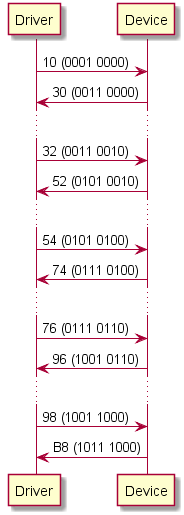
\includegraphics[scale=1.0]{out/FrameI_Bajt_kontrolny/FrameI_Bajt_kontrolny.png}
\caption{Ramka informacyjna - ewaluacja bajtu kontrolnego}
\end{figure}

  \chapter{SOLID}
Projektując sterownik podjęto próbę podążania zgodnie z dobrymi praktyk programowania, powszechnie znanymi jako SOLID.
Pomyślna ich realizacja sprawia, że korzystanie, rozbudowywanie jak i utrzymywanie powstałego kodu źródłowego przypomina
przyjemne poruszanie się po świecie gry aniżeli walkę z napotkałymi przeszkodami. 
Tak powstały program umożliwia łatwe ponowne używanie wcześniej powstałego kodu. 
Zwrócić też trzeba uwagę na użyte wcześniej słowo, gdyż nie przez przypadek wspomniałem właśnie o dążeniu do ich wdrożenia.
Poniższe reguły czasami bywają ciężkie w realizacji zwłaszcza, kiedy nasz system osiągnie duże rozmiary, dlatego warto myśleć o nich już na początkowym etapie. 
Trzeba też pamiętać o tym, że nie jest rozsądne stosowanie którejkolwiek z reguł SOLID, jeśli nie ma ku temu wyraźnych powodów, dlatego 
jedynie doświadczenie oraz intuicja pozwoli nam wyczuć moment podjęcia decyzji projektowej.
Pozwolę sobie przedstawić prawa budujące zasady SOLID oraz wspomnieć o ich głównych założeniach.

\section{SRP}
Z angielskiego Single Responsibility Principle, a więc zasada pojedynczej odpowiedzialności.
Mówi ona, że powód modyfikacji klasy powinien być tylko jeden. \autocite[103]{martin2015zwinne}
Realizacja tej reguły uchroni nas przed niechcianą modyfikacją definicji dużej liczby klas w przypadku zmiany logiki tylko jednej z nich.

\section{OCP}
Z angielskiego Open/Closed Principle, a więc zasada otwarte-zamknięte.
Mówi ona, że encje programowanie (klasy, moduły, funkcje itp.) powinny być otwarte na rozbudowę, ale zamknięte dla modyfikacji.\autocite[117]{martin2015zwinne}
Jeśli ta zasada zostanie właściwie zastosowana, to nowe zmiany uzyskuje się poprzez dodanie nowego kodu, aniżeli zmiane istniejącego. 

\section{LSP}
Z angielskiego Liskov Substitution Principle, a więc zasada podstawiania Liskov.
Mówi ona, że musi być możliwość podstawienia typów pochodnych za ich typy bazowe.\autocite[127]{martin2015zwinne}
Trzeba pamiętać o tej regule w trakcie definiowania relacji dziedziczenia pomiędzy klasami.

\section{ISP}
Z angielskiego Interface Segregation Principle, a więc zasada segregacji interfejsów.
Mówi ona, że klienty nie powinny być zmuszone do zależności od metod, których nie używają.\autocite[151]{martin2015zwinne}
Dzięki postępowaniu zgodnie z tą zasadą, utworzone interfejsy abstrakcyjnych klas bazowych będą zawierały minimalną liczbę funkcji czysto wirtualnych.

\section{DIP}
Z angielskiego Dependency Inversion Principle, a więc zasada odwracania zależności.
Mówi ona, że moduły wysokopoziomowe nie powinny zależeć od modułów niskopoziomowych. I jedne, i drugie powinny zależeć od abstrakcji.\autocite[141]{martin2015zwinne}
Kolejnym postulatem jest to, że abstrakcje nie powinny zależeć od szczegółów. To szczegóły powinny zależeć od abstrakcji.\autocite[141]{martin2015zwinne}


  \part{Część Praktyczna}
  \chapter{Wzorce projektowe}
W latach, kiedy programowanie obiektowe stawało się bardziej popularne, wiele osób natrafiało na grupę problemów pewnej kategorii.
Podczas wielokrotnych prób ich rozwiązywania, różne osoby dochodziły do wspólnych wniosków odnośnie do architektury kodu źródłowego tworzonego w celu ich rozwiązania.
Napotykane wyzwania rozpoczęto dzielić według trzech kategorii: behawioralne, strukturalne oraz kreacyjne. Tak oto to powstały wzorce projektowe.
Obszerna znajomość tej niemałej dziedziny informatyki pozwala spojrzeć na kolejne zadania w znacznie bardziej zaawansowany sposób aniżeli wcześniej.
Można je porównać do znanych przekształceń oraz wzorów matematycznych w rachunku całkowym, gdyż zostały one ściśle zdefiniowane, a osiągniecie efektu końcowego różni się
zastosowanie innych parametrów wejściowych. Podczas tworzenia wzorców usilnie trzymano się zbioru kolejnych zasad znanych pod nazwą SOLID. \newline
Poniżej przedstawiono użyte podczas projektowania sterownika wzorce wraz z fragmentami kodu źródłowego.
\section{Behawioralne}
    \subsection{Komenda}
        Dzięki utworzeniu interfejsu komendy, zrealizowano regułę otwarcia na modyfikacje a zamknięcia na zmiany.
        W przypadku poprawnej definicji funkcjonalności, która powinna zostać zrealizowana, dodajemy jedynie implementację tego interfejsu,
        przez co cała regresja pozostaje bez zmian, a dzięki kontrolerowi, który kolejkuje komendy można pokusić się o realizację kompozytu oraz
        wprowadzenie systemu wag bądź poleceń terminujących aktualnie zaplanowane zadania.
        Podczas implementacji sterownika zastosowano połączenie trzech wzorców projektowych a to wszystko dzięki potężnemu podejściu do organizacji
        struktury kodu jakim jest użycie komend. Zestawiając implementację interfejsu komendy oraz budowania konkretnej wiadomości dzięki fabryce
        pozwala na zdefiniowanie \textit{klas finalnych} zawierających charakterystyczne dla każdej z komend wywołań. 
    \newpage
        \lstinputlisting[
            language=C++,
            caption=Interfejs komendy]
            {Kod_Zrodlowy/DesignPatterns_Command_1.cpp}
        \lstinputlisting[
            language=C++,
            caption=Definicja klasy konkretnej komendy używającej fabryki oraz strategii]
            {Kod_Zrodlowy/DesignPatterns_Command_2.cpp}
        \begin{figure}[h!]
            \centering
            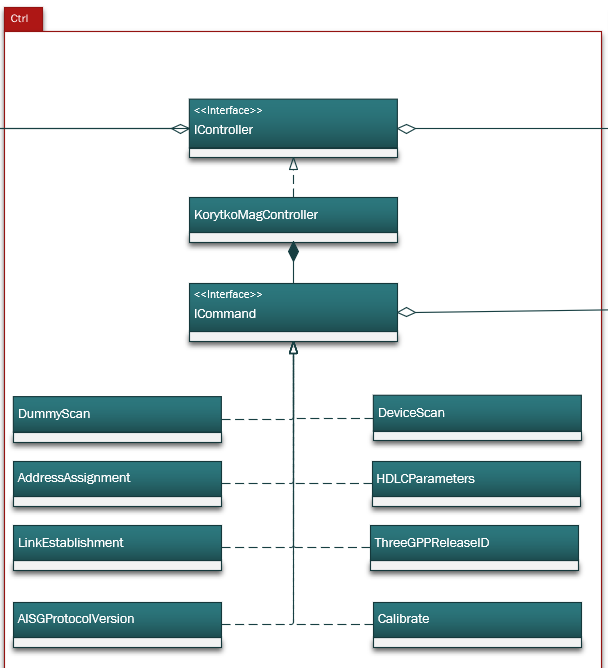
\includegraphics[scale=0.90]{Obrazki/DiagramyKlas/Ctrl.png}
            \caption{Diagram klas przedstawiający realizację wzorca komendy.
                \newline(Opracowanie własne)}
        \end{figure}
    \newpage
    \subsection{Obiekt pusty}
        Znaną przypadłością w językach obiektowych jest wykonywanie dalszej akcji w zależności od stanu pewnego z obiektów.
        W przypadku korzystania ze wskaźników dobrą praktyką jest każdorazowa weryfikacja czy jego wartość nie jest równa \textit{null}.
        Wykorzystanie klasy która implementuje interfejs kontrolera, w sposób neutralny sprawia, że zawsze bezpieczne będzie wywołanie na jej obiekcie 
        instancjonującym którejkolwiek z metod.
    \newpage
        \lstinputlisting[
            language=C++,
            caption=Definicja klasy dla obiektu pustego]
            {Kod_Zrodlowy/DesignPatterns_NullObject_Implementation.cpp}
        \lstinputlisting[
            language=C++,
            caption=Przykład użycia obiektu pustego]
            {Kod_Zrodlowy/DesignPatterns_NullObject_Usage.cpp}
    \newpage
    \subsection{Metoda szablonowa}
        Wprowadzenie systemu walidacji argumentów podanych przez użytkownika gwarantuje bezpieczne wykonywanie akcji niskopoziomowych takich
        jak wysłanie wiadomości do urządzenia, bez zbędnego umieszczanie logiki weryfikacji w dalszym etapie. Zastosowanie tego wzorca umożliwi w przyszłości wdrożenie dodatkowych mechanizmów.
        Jednym z nich jest automatycznie pobranie długiego adresu portu na który ma zostać wysłana komenda, w przypadku podaniu klucza obiektu w bazie danych. 
        Natomiast następnym jest funkcjonalność automatycznej korekty w przypadku zaistniałego błędu syntaktycznego we wprowadzanej przez użytkownika komendzie.
        Obecność komendy ,,execute'' pozwala połączyć wywołanie powyższych funkcji za pomocą jednego polecenia,
        nie posiadając wiedzy o tym jakiego typu procedury weryfikacji sterownik będzie próbował dokonać. Powyższą funkcjonalność osiągnięto dzięki efektownemu wykorzystaniu
        funkcji wirtualnych.
        \lstinputlisting[
            language=C++,
            caption=Plik nagłówkowy dla metody szablonowej walidacji komendy]
            {Kod_Zrodlowy/DesignPatterns_TemplateMethod_Header.hpp}
        \lstinputlisting[
            language=C++,
            caption= Metoda szablonowa - Wywołanie metod wirtualnych z poziomu innej metody]
            {Kod_Zrodlowy/DesignPatterns_TemplateMethod_Implementation.cpp}
    \subsection{Strategia}
        Znanych jest wiele wzorców komunikacji pomiędzy komponentami aczkolwiek w projekcie użyto dwa najbardziej znane: Publikuj-Subskrybuj oraz Żadanie-Odpowiedź.
        
        \begin{figure}[h!]
            \centering
            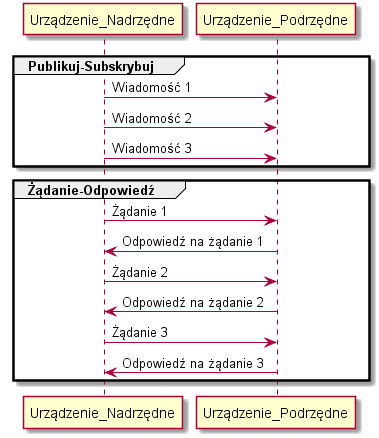
\includegraphics[scale=0.75]{out/Diagramy/PublishSubscribe_RequestResponse.png}
            \caption{Przepływ wiadomości dla wzorca Publikuj-Subskrybuj oraz Żądanie-Odpowiedź.
                \newline(Opracowanie własne)}
        \end{figure}

        Pierwszy z nich efektownie realizuje zasadę odwrócenia zależności, ponieważ sterownik urządzenia nadrzędne na początkowym etapie nie musi znać
        ilości podłączonych do linii urządzeń. Drugi namiast pozwala zrealizować podejście do transmisji z urządzeniem znane jako półdupleks, wymagane podczas
        wywoływania komend zestawiających warstwę łącza danych oraz aplikacyjnej. Głównym problem jest to, że obydwa wzorce wymagają innego zestawu komend w celu
        konfiguracji połączenia ze slotami systemowymi. W projekcie zaimplementowano jeden kontroler, który zarządza zestawianiem wymaganych warstw OSI w trakcie
        ciągłego uruchomienia sterownika, co osiągnięto dzięki dynamicznemu podmianie strategii komunikacji z Publikuj-Subskrybuj na Żadanie-Odpowiedź.
        Zaobserwowano pewne złe następstwo niepoprawnego użycia wzorca strategii polegające na prewencyjnemu rzuceniu wyjątku w przypadku gdyby programista wywołał niepoprawną metode.
        W związku z tym, podczas przyszłej rozbudowy programu, zastosowany zostanie inny wzorzec o nazwie most.
        \newpage
        \lstinputlisting[
        language=C++,
        caption=Strategia komunikacji Żadanie-Odpowiedź dla urządzenia nadrzędnego]
        {Kod_Zrodlowy/DesignPatterns_Strategy.cpp}
    \newpage
    \subsection{Wstrzykiwanie zależności}
        Klasa ,,HDLCCommand'' bezpośrednio dziedziczy po klasie ,,Command''. Dzięki implementacji interfejsu ,,execute'' zrealizowany kontroler posiada możliwość,
        przyszłej rozbudowy nawet o komendy typu ,,włącz muzykę''. W przypadku obsługi urządzenia implementującego protokół AISG, zaobserowowano zapotrzebowanie
        na dodatkową klasę abstrakcyjną, która posiadała będzie wskaźnik na obiekt implementujący interfejs fabryki ramek oraz wzorca komunikacji.
        Podejście programowania sterowanego testami umożliwiło przedstawienie programisty przed koniecznością przekazania powyższych obiektów z poziomu testu, w celu wyeliminowania
        wymagania podłączania fizycznego urządzenia bądź uruchamiania aplikacji symulującej urządzenie oraz skrócenia czasu regresji programu, dzięki
        korzystaniu z atrap.
        Ten sposób zarządzania kolejnością tworzenia oprogramowania naturalnie wymusił realizację wstrzykiwania zależności polegającej na
        przekazywaniu obiektów z zewnątrz podczas wywoływania konstruktora, aniżeli utworzeniu konstruktora zeroparametrowego, 
        który uniemożliwia dalszą modernizacjię elementów składowych systemu.
        \lstinputlisting[
        language=C++,
        caption=Konstruktor zrealizowany podejściem wstrzykiwania zależności]
        {Kod_Zrodlowy/DesignPatterns_DependencyInjection.cpp}
    \subsection{Inicjowanie przy pozyskaniu zasobu}
        Do implementacji pracy użyto kompilator GCC wspierający język C++ w wersji 11-tej, który posiada wbudowany mechanizm inteligentnych wskaźników. ,,shared\_ptr<T>'' oraz ,,unique\_ptr<T>''
        zmieniły sposób korzystania z dynamicznie alokowanej pamięci w sposób diametralny. Do tej pory dealokacja pamięci wskazywanej przez wskaźnik należała do obowiązków programisty.
        Dzięki podejściu tzw. RAII dla ,,shared\_ptr<T>'', w przypadku destrukcji wszystkich wskaźników odnoszących się do wcześniej zaalokowanego obszaru pamięci,
        kompilator przy pomocy destruktora wywołuje komendę ,,delete'' automatycznie, dzięki czemu programista jest ustrzeżony przed niepożądanym wyciekiem pamięci.
\newpage
\section{Kreacyjne}
    \subsection{Budowniczy}
        Często zdarza się, że obiekt klasy wymaga modernizacji wielu z jego pól a realizacja konstruktora posiadającego trzy bądź więcej parametrów,
        uznawana jest za niepoprawną implementacje oraz antywzorzec. W tej sytuacji z pomocą pojawia się wzorzec budowniczego, który podczas wywoływania metody 
        zmieniającej stan obiektu, dokonuje zamierzonego celu, po czym zwraca referencję na obiekt na rzecz którego została wywołana \textit{metoda}. 
        Umożliwia to szeregowe wywoływanie kolejnych modyfikatorów co znacznie oczyściło i zwiększyło czytelność programu. Istnieje wiele interpretacji tego wzorca projektowego,
        w których dodana jest metoda finalizująca budowanie obiektu.
        \lstinputlisting[
            language=C++,
            caption=Budowniczy wraz z Fluent API podczas budowania ramki I - Kalibruj]
            {Kod_Zrodlowy/DesignPatterns_Builder.cpp}
\newpage
    \subsection{Fabryka}
        Istnieje pewien wzorzec, który owiany jest złą sławą. Programiści w momencie usłyszenia o nim dostają ciarek, gdyż sądzą, że pod tym słowem,
        kryje się obiekt, który potrafi zachować się w nieprzewidziany sposób podczas każdorazowego wywoływania jego metod. Z drugiej strony poprawna jego realizacja, 
        umożliwia dynamiczną zmianę wartości zwracanych przed system, a w przypadku sterownika dała możliwość uwspólnienie kodu wraz z symulatorem urządzenia,
        na poziomie 90\%. Mowa o fabryce. W przypadku nieprzechowywania jakiegokolwiek stanu w jej instancji oraz zapoznania się w całości z realizowanym problemem
        komunikacji pomiędzy urządzeniem podrzędnym i nadrzędnym, prawdą jest to, że zaledwie na jedną komendę sterownik nie oczekuje odpowiedzi, a odpowiednie
        nazwanie metod interfejsu fabryki pozwoli zaobserwować, że po obu stronach trzeba obsłużyć komunikację oraz budowę wiadomości charakterystyczną na przykład
        dla polecenia ,,kalibruj'' wprowadzając jedynie niewielkie modyfikacje. 
        \lstinputlisting[
        language=C++,
        caption=Fabryka budowniczych dla sterownika urządzenia nadrzędnego]
        {Kod_Zrodlowy/DesignPatterns_Factory.cpp}

  \chapter{Wymagania funkcjonalne}
	\section{Historyjki użytkownika ( Warstwa fizyczna łącza danych ) - nazwa komendy}
		Proces nawiązania połączenia z RET-em można zamodelować przy pomocy maszyny stanów w związku z czym z poniższych funkcjonalności należy korzystać zgodnie z zadaną kolejnością.
		Dla każdej z poniższych ramek wyznaczono część wspólną składającą się z czterech bajtów. Pierwszym z nich jest bajt flagi startu, która oznacza początek wiadomości i ma wartość 0x7E.
		Koleje bajty budują ramkę XID, I, U, S o których wspomniano wcześniej. Następnie dodaje się dwubajtową sumę CRC oraz na samym końcu flagę stopu, która jest tej samej wartości co flaga startu i oznacza koniec nadawania wiadomości.
		\subsection{Ustanowienie prędkości połączenia - SetLinkSpeed}
			Jako użytkownik chcę ustawić jeden z parametrów warstwy fizycznej a mianowicie prędkość transmisji równą 9.6 kbps.
			\newline\newline
			Jest to komenda wysyłana do urządzenia podrzędnego przy pomocy ramki XID.
			\newline
			Pierwsze dwa bajty o wartości 0xFF odpowiadają za zdefiniowanie adresu urządzenia docelowego. 
			W tym przypadku celem jest synchronizacja prędkości połączenia ze wszystkimi urządzeniami na lini, które nie są zaadresowane a więc jest to wiadomość typu ,,broadcast''.
			\newline
			Kolejne dwa bajty kontrolne o wartości 0xBF są charakterystyczne dla ramki XID.
			\newline
			Następne dwa bajty o wartości 0x81 identyfikują format wiadomości XID, co oznacza że jest to wiadomość z kategorii przypisania adresu.
			\newline
			Potem napotykamy kolejne dwa bajty o wartości 0xF0 które są identyfikatorem grupy, co mówi nam jakie kolejne bajty dopuszczalne są w dalszej części wiadomości.
			\newline
			Urządzenie podrzędne w celu umożliwienia mu zdekodowania wiadomości, otrzymuje w wiadomości długość grupy, czyli dwa bajty w tym przypadku o wartości 0x08 i jest to 
			liczba bajtów która pojawi się następnie, aż do sumy CRC i bajtu stopu.
			\newline
			Przechodząc do przesyłanych parameterów, jako pierwszy będzie to unikalny identyfikator urządzenia. Możemy to rozpoznać po identyfikatorze o wartości 0x01.
			Następnie podajemy liczbę bajtów zajmowanych przez UniqueID czyli 0x02. Kolejnie podajemy wartość unikalnego identyfikatora. Z racji tego, że nie oczekujemy odpowiedzi
			na tę wiadomość, są to dowolne wartości.
			Drugim przesyłanym parametrem jest maska danych z identyfikatorem o wartości 0x03, potem podajemy liczbę bajtów budujących przesyłaną przez nas maskę czyli 0x02, a w wartości 
			parametru umieszczamy 4-ry bajty o wartości obu 0xFF. Jest to najbardziej ogólna maska urządzenia.
		\subsection{Negocjacja roli - AddressAssignment}
			Jako użytkownik chcę zaadresować urządzenie typu SingleRET identyfikujące się unikalnym identyfikatorem\footnote{\label{UniqueID} UniqueID - Dla AISG v2.0 jest to złożenie numeru seryjnego wraz z kodem producenta} == \{0x4E, 0x4B, 0x34, 0x36, 0x35, 0x30, 0x30, 0x30, 0x30\} adresem 3, 
			przy pomocy komendy ,,AddressAssignment''.
			\newline\newline
			Budowa ramki wysyłanej przez tę komendę jest bardzo podobna do powyższej z racji tego, że powyższą można nazwać atrapą skanu a tą skanowaniem celowanym.
			Z racji tego, że różna jest liczba oraz wielkość poszczególnych parametrów HDLC, bajt rozmiaru grupy posiada wartość 0x11.
			\newline
			Pierwszy parametr identyfikuje się przy pomocy wartości 0x01 czyli jest to unikalny identyfikator urządzenia, który ma zostać zaadresowany.
			Kolejny bajt przypomina o rozmiarze parametru i w tym przypadku jest on równy 0x09. W powyższym opisie przedstawiono unikalny identyfikator urządzenia, który w przypadku
			równości z rzeczywistym, pozwala urządzeniu podrzędnemu przyjąć żądanie adresacji.
			\newline
			Następny parametr posiada wartość 0x02 i oznacza on, że w jego wartości urządzenie nadrzędne zdefiniowało adres urządzeniu wewnetrznemu, dzięki któremu
			będzie identyfikowane oraz z racji tego, że długość parametru ma wartość 0x01, to wartość wynosi 0x03. W przypadku projektu, nie będzie miał on większego znaczenia
			aczkolwiek w momencie kiedy urządzenia typu Ret połączone są ze sobą szerogowo, potrzeba jest możliwość wysłania wiadomości do na przykład drugiego w łańcuchu.
			\newline
			Ostatnim parametrem jest 0x04 który mówi nam o tym, że urządzenie nadrzędne uważa, że po drugiej stronie jest jedno z urządzeń zdefiniowanych 
			według standardu AISG 2.0, w tym przypadku długość również wynosi 0x01 a wartość to 0x01. Oznacza ona, że próbujemy nawiązać komunikację z pojedyncznym RET-em.
			Dla porównania istnieją również urządzenia takie jak MultiRET, dzięki któremu można zmieniać wartość nachylania kąta głównej wiązki anteny na wielu osiach czy płaszczyznach.
		\subsection{Negocjacja parametrów HDLC - HDLCParameters}
			Jako użytkownik chcę ustalić maksymalny rozmiar nadawanej jak i odbieranej ramki typu I oraz maksymalną ilość ramek jednocześnie możliwych do wysłania bądź odebrania.
			\newline\newline
			Powyższą wiadomość można rozbić na 4-ry osobne aczkolwiek połączono je z racji podobnych funkcjonalności realizowanych podczas jej wysłania. Protokół AISG bazuje na HDLC, które używane jest w wielu miejscach
			gdzie potrzebne jest połączenie połączenie o wysokiej gwarancji otrzymania wiadomości bez utraty informacji. Istnieje nawet jego realizacja służąca do komunikacja satelit kosmicznych i różni się ona od AISG głównie
			ustalonymi wiadomościami HDLC, gdzie potrzeba wysłać znacznie większą liczbę ramek na raz aniżeli tylko jedna.
			Pierwszy bajt adresu może zostać zmieniony z wartości 0xFF na 0x03, gdyż w poprzedniej wiadomości ustanowiono adres urządzenia podrzędnego. Ta wartość będzie aplikowana do każdej poniższej wiadomości a więc pominięto jej wspominanie,
			gdyż potraktowano ją jako stałą.
			\newline
			Następnym bajtem jest identyfikator formatu, który dla wiadomości zawierającej parametry HDLC jest równy 0x81.
			\newline
			Kolejny bajt czyli identyfikator grupy ma wartość 0x80, a następny (rozmiar grupy) jest równy 0x12.
			\newline
			Pierwszym parametrem HDLC który jest negocjowany to maksymalny rozmiar tzw. payloadu dla ramki informacyjnej nadawanej przez urządzenie nadrzędne. Identyfikatorem w tym przypadku jest 0x05. Rozmiar payloadu jest równy 0x04 a wartościami są \{ 0xF0, 0x2D, 0x00, 0x00 \}.
			\newline
			Kolejny bajty natomiast budują negocjowany maksymalny rozmiar payloadu ramki informacyjnej do wiadomości otrzymywanej przez urządzenie nadrzędne. Identyfikator ma wartość 0x06 a pozostały bajty są tożsame jak dla poprzedniej
			negocjacji.
			\newline
			Następnym parametrem jest maksymalna liczba ramek wysłanych pod rząd przez urządzenie nadrzędne. Identyfikator ma wartość 0x07 a zarówno długość jak i wartość to 0x01.
			\newline
			Ostatnim parametrem negocjowanym podczas tej wiadomości jest maksymalna liczba ramek otrzymanych pod rząd poprzez urządzenie nadrzędne. Wartość identyfikatora jest równa 0x08 a długość oraz wartość znów posiadają wartości 0x01.
		\subsection{Ustanowienie synchronicznego trybu komunikacji - LinkEstablishment}
			Jako użytkownik chcę ustawić synchroniczny tryb komunikacji z urządzeniem.
			\newline\newline
			Bajt kontrolny posiada wartość 0x93 i oznacza żadanie ustalenia sposobu komunikacji z urządzeniem podrzędnym na tryb normalny, a więc taki w którym wysyła ono ramkę jedynie jako odpowiedź
			na wcześniej nadaną przez urządzenie nadrzędne.
		 \subsection{Negocjacja parametrów HDLC - 3GPPReleaseID}
			Jako użytkownik chcę wynegocjować parameter HDLC urządzenia, jakim jest wspierana wersja 3GPP. \newline
			\newline\newline
			Teraz można przejść do coraz bardziej szczegółowych parametrów jak ustanowienie numeru wersji standardu 3GPP.\footnote{\label{3GPP} 3GPP - 3rd Generation Partnership Project, komisja standaryzacyjna która tworzy protokoły telekomunikacyjne.}
			Podczas tworzenia tej wiadomości znów skorzystano z ramki XID a więc należy zdefiniować identyfikator formatu, grupy oraz jej długość. Pierwsze dwie wartości są równe tym z komendy ,,AddressAssignment'' a długość ma wartość 0x03.
			Identyfikatorem parametru jest tym razem wartość 0x05, długością 0x01 natomiast wartościa parametru 0x08. Jest to wersja standardu w wersji 8-mej czyli pionierska dla technologii LTE\footnote{\label{LTE} LTE - Long term evolution.}.
			Wprowadzono w niej wparcie dla interfejsu radiowego opartego o OFDMA\footnote{\label{OFDMA} OFDMA - Orthogonal frequency-division multiple access.}, którego wykorzystanie można zaobserwować również przy technologii 5G.
		\subsection{Negocjacja parametrów HDLC - AISGProtocolVersion}
			Jako użytkownik chcę wynegocjować parameter HDLC urządzenia, jakim jest wspierana wersja protokołu AISG. \newline
			Z racji tego, że aktualną wersją protokołu AISG jest ta z numerem 2.0, istnieją jeszcze dwie wcześniejsze jak 1.0, 1.1 oraz w trakcie wdrażania jest również 3.0, potrzeba zdefiniować według którego standardu budowane są
			wiadomości przez urządzenie nadrzędne oraz rozpoznawane przez podrzędne.
			Bajt identyfikujący parametr dla tej wiadomości ma wartość 0x14, długość parametru to 0x01 a jej wartość to 0x02.
	\section{Historyjki użytkownika ( Warstwa aplikacyjna ) - nazwa komendy}
		Po pomyślnym zestawieniu warstwy fizycznej posiadamy zdefiniowany wszystkie charakterystyki połączenia, które pozwolą w jednoznaczny sposób porozumieć sie z urządzeniem oraz żądać odpowiedzi na wysłaną wiadomość.
		Kolejne komendy są już żądaniami wysokoziomowymi, które definiują użyteczne dla klienta polecenia służąca do zarządzania RET-em. Jest ich znacznie więcej, aczkolwiek obranym celem pracy inżynierskiej było pomyślne przeprowadzenie
		kalibracji urządzenia, co pozwala w dalszym etapie ustawić zadany kąt odchylenia głównej wiązki sygnału z anteny.
		\subsection{Kalibracja - Calibrate}
			Jako użytkownik chcę skalibrować urządzenie.
			\newline\newline
			Z racji tego, że wiadomości tej warstwy korzystają z ramki informacyjnej, inną rolę pełni bajt kontrolny. Poza stałymi wartości bitów w bajcie, każdorazowe wysłanie i odebranie wiadomości zmienia wartość sekcji P/F wcześniej wspomnianej. Dzięki temu można w łatwy sposób identyfikować czy wiadomość którą otrzymujemy jest ta której oczekiwaliśmy. W związku z tym dla pierwszej wiadomości wysłanej przez urządzenie nadrzędne poprawną wartością, będzie
			0x10.
			\newline
			Kolejnym bajtem jest kod procedury, który ma wartość 0x31, co oznacza, że oczekujemy kalibracji urządzenia będącego zwykłym pojedynczym RET-em.
			\newline
			Z racji tego, że podczas tej komendy nie jest przesyłana żadna wartość dla tej procedury, dwa bajty zaalokowane dla długości parametru posiadają wartość \{0x00, 0x00\}

  \section{Uruchomienie programu}
    \begin{enumerate}
        \item Uruchomienie systemu Manjaro Linux;
        \item Podłączenie do internetu w celu pobrania repozytorium;
        \item Konfiguracja środowiska (pomiń w przypadku posiadania kompletu):
        
            \item sudo cmake
            \item cmake
        \item otwarcie pierwszej konsoli oraz wywołanie poniższych komend, w celu uruchomienia symulatora urządzenia:
		\begin{enumerate}
			\item ,,git clone https://github.com/trunksBT/KorytkoMag\_RetSimulator.git -{}-recursive''
			\item ,,cd KorytkoMag\_RetSimulator''
			\item ,,make .''
			\item ,,bash runBinary.sh''
		\end{enumerate}
		\item otwarcie drugiej konsoli, w celu uruchomienia sterownika:
		\begin{enumerate}
			\item ,,git clone https://github.com/trunksBT/KorytkoMag\_RetDriverSimulator.git -{}-recursive''
			\item ,,cd KorytkoMag\_RetDriverSimulator''
			\item ,,make .''
			\item ,,bash runBinary.sh''
			\item Wywołanie komend zgodnie z diagramem sekwencji zatytułowanym ,,KalibracjaRETa''
			\item Aby zakończyć trzeba wpisać ,,exit''
		\end{enumerate}
    \end{enumerate}

  \include{czescPraktyczna_analizaNawiazanejKomunikacji}
  \chapter{Logi z wykonania}
    \section{Program właściwy}
        \lstinputlisting[
        language=bash,
        basicstyle=\tiny,
        caption=Działanie sterownika]
        {LogZWykonania/BinaryLog.log}
    \section{Test jednostkowe}
        \lstinputlisting[
        language=bash,
        basicstyle=\tiny,
        caption=Testy jednostkowe]
        {LogZWykonania/LogsFromUT.log}
    \section{Test modułowe}
        \lstinputlisting[
        language=bash,
        basicstyle=\tiny,
        caption=Testy modułowe]
        {LogZWykonania/LogsFromMT.log}
        
  \chapter{Wymagania niefunkcjonalne}
\section{Środowisko uruchomieniowe}
	\begin{itemize}
		\item System operacyjny Linux
			\begin{itemize}
				\item Dystrybucje:
				\begin{itemize}
					\item Manjaro 17.01;
				\end{itemize}
				\item Zależności:
					\begin{itemize}
						\item CMake 3.15.4;
						\item Boost C++ Libraries 1.71;
						\item Git -> Pobranie kodu produkcyjnego, GTest, GMock;
						\item GCC 9.2;
					\end{itemize}
			\end{itemize}
		\item Podłączenie do internetu w celu pobrania repozytorium oraz kompilacji programu uruchomieniowego
		\item Instalacja
		\begin{enumerate}
			\item git clone https://github.com/trunksBT/Almag\_RetDriverSimulator.git -{}-recursive
			\item cd Almag\_RetDriverSimulator
			\item make .
			\item bash runBinary.sh
		\end{enumerate}
	\end{itemize}
\section{Zrzuty ekranu}
	\begin{figure}[p]
	\includegraphics[scale=0.3]{ExecutionOfMT.png}
	\caption{Zrzut ekranu z wykonania testów modułowych}
	\end{figure}
	
	\begin{figure}[p]
	\includegraphics[scale=0.3]{ExecutionOfUT.png}
	\caption{Zrzut ekranu z wykonania testów jednostkowych}
	\end{figure}
	
	\begin{figure}[p]
	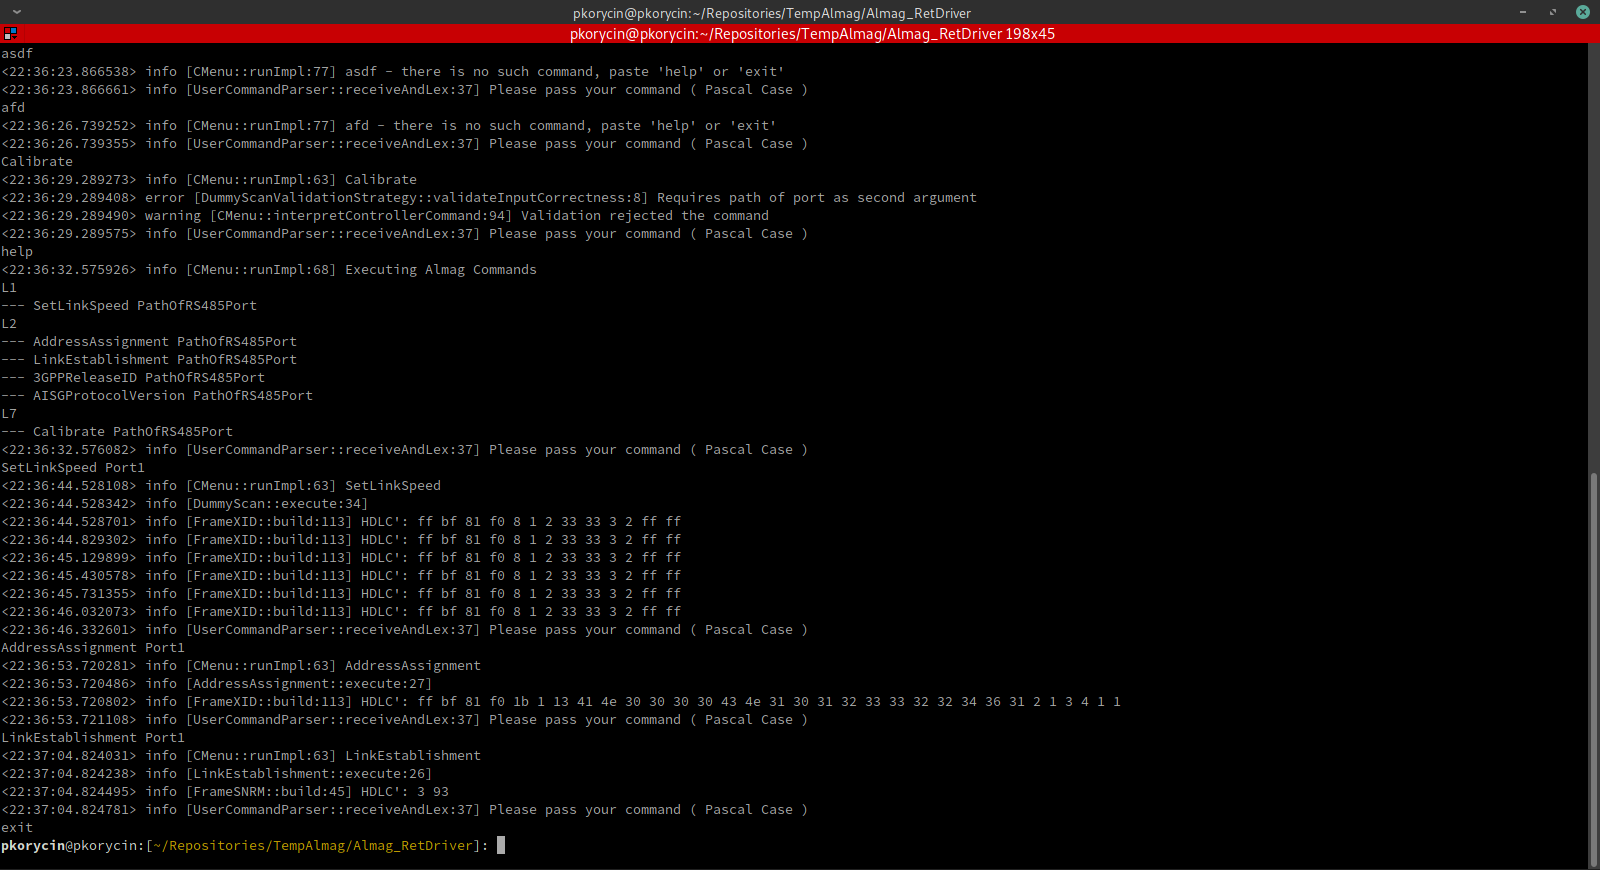
\includegraphics[scale=0.3]{ExecutionOnSeverityInfo.png}
	\caption{Zrzut ekranu z uruchomienia programu z odfiltrowaniem logów poniżej priorytetu info}
	\end{figure}
	
	\begin{figure}[p]
	\includegraphics[scale=0.3]{ExecutionOnSeverityTrace.png}
	\caption{Zrzut ekranu z uruchomienia programu bez odfiltrowania logów}
	\end{figure}


  % \chapter{Plan dalszego rozwoju}
\section{Porażki odnośnie planu początkowego}
    W celu przesłania wiadomości zapisanej w systemie heksadecymalnym przy pomocy interfejsu USB <-> RS-485
    należy dokonać konwersji na postać binarną. Zarówno wiadomość odebrana jak i wysłana może w trakcie transmisji ulec wybrakowaniu bądź
    zmianie zawartości. W tym celu ramka HDLC posiada bajt bądź dwa bajty przeznaczone na walidację takowej wiadomości, w przypadku protokołu
    AISG 2.0 jest to suma CRC. W związku z tym, że istnieje wiele implementacji algorytmu wyliczania sumy CRC a każda z nich może różnić się od siebie zarówno:
    definicją wyrażenia wielomianowego, jego postacią oraz wartością początkową, próbowałem na podstawie ,,podsłuchanej'' wiadomości przy pomocy
    inżynierii wstecznej zdefiniować brakującą wiedzę, lecz aby tego dokonać potrzebowałem więcej informacji na temat zarówno endianowości
    jak i uporządkowania bitów dla poszczególnych ramek HDLC a pomimo tego, że dla komputera jest to prosta operacja, to weryfikacja przez człowieka
    wartości sumy CRC dla wiadomości o długości 16-tu bajtów na kartce zajmuje naprawdę dużo czasu. W dodatku powszechnym problemem jest to, że 
    producenci urządzeń linii antenowej pomimo tego, że deklarują pełną implementację protokołu AISG 2.0, to w rzeczywistości okazuje się, że
    wcale tak nie jest. Chcąc zapoznać się z protokołem komunikacyjnym oraz zrealizować projekt inżynierski podczas którego sprawdzę umiejętności testowania,
    wdrażania wzorców projektowych czy też posługiwania się językiem C++ zamiast walczyć z urządzeniem i jego możliwymi błędami, postanowiłem
    utworzyć symulator urządzenia, który będzie komunikował się przy pomocy biblioteki ZeroMQ. Dzięki zaznajomieniu się z wieloma wzorcami projektowymi
    jak fabryka, komenda, budowniczy czy nakładanie obostrzeń na program dzięki listowaniu obsługiwanych komend, wspomniany wcześniej
    symulator urządzenia powstał niemalże za darmo, co uznaję za bardzo duży sukces z dziedziny projektowania architektury oprogramowania.
    Kolejną zaletą utworzenia symulatora urządzenia jest umożliwienie testów komponentowych realizując regułę czarnej skrzynki, co pozwoli w przyszłości
    znacznie skrócić czas testowania sterownika pod względem błędów logicznych.
\subsection{Weryfikacja wiadomości pod względem obecności zarezerwowanych znaków}
    Z języka angielskiego ,,Byte stuffing''. Procedura polega na tym, że zarówno flaga startu jak i stopu posiadają zarezerwowaną wartość 0x7E.
    Niestety urządzenie podrzędne może odpowiedzieć na przykład podczas procedur XID negocjacji, wiadomością zawierającą bajt 0x7E. Nieobsłużone
    takie zjawisko spowoduje, że urządzenie nadrzędne zinterpretuje ten bajt jako bajt stopu, co jest niepożądane. W tym celu standard AISG 
    definiuje procedurę do jakiej należy się zastosować w takiej sytuacji, z którą nie zaznajomiłem się.
\subsection{Interwały czasowe}
    Protokół AISG 2.0 definiuje szereg interwałów których obecność można zaobserwować podczas komunikacji z urządzeniem. Jednym z nich jest
    utrzymanie urządzenia w stanie zaadresowanym. W przypadku kiedy urządzenie podrzędne nie otrzyma jakiejkolwiek wiadomości w przeciągu 3 minut
    od jego zaadresowania, przechodzi ono w stan niezaadresowany, po czym ponownie należy zestawić warstwę fizyczną oraz łącza danych wraz
    z całą procedurą XID negocjacji. Kolejnymi zależnościami czasowymi są odstępy pomiędzy wysłaniem wiadomości a rozpoczęciem nasłuchiwania na odpowiedź.
    Problemem mógłby być scenariusz w którym wysyłamy wiadomość do urządzenia podrzędne jest ono na przykład w trakcie procedury kalibracji która może 
    trwać ok 2 minuty. Jako odpowiedź możemy wtedy otrzymać ramkę typu S której stan rozpoznamy jako odpowiedź RNR z angielskiego Receiver Not Ready. 
    W tej sytuacji należy odczekać pewien kwant czasu a następnie ponowić komunikację.
\subsection{Ustalanie maski}
    RetSimulatorjest urządzeniem które często posiada wbudowane wejście RS-485 out, co oznacza
    że można podłączyć dwa bądź więcej urządzeń szeregowo. W takiej sytuacji na wiadomość pochodzącą z nadrzędne
    zaadresowaną wartością równą 0xFF, każde z nich wyśle swoją odpowiedź co niesie ze sobą wiele problemów.
    Po stronie urządzenia nadrzędne zaobserwujemy to w ten sposób, że nasłuchiwane w czasie standardowego interwału czasu bajty
    pochodzić będą naprzemian od dwóch różnych urządzeń. Algorytm definiowania maski skutecznie rozwiązuje ten problem. 
    Podczas tej procedury dążymy do ustalenia unikalnego identyfikatora każdego z urządzeń, w celu wysłania wiadomości z żadaniem zaadresowania,
    na którą odpowie tylko jedno urządzenie. Realizacja powyższego problemu często korzysta z algorytmów przeszukiwania binarnego w trakcie którego
    zadaniem jest ustalenie unikalnego identyfikatora na którego składa się numer seryjny oraz kod producenta. Z racji tego, że podczas pracy inżynierskiej
    przewidywano uruchomienie instancji sterownika dla każdego urządzenia osobno, pominięto implementację wyżej wymienionej logiki.
\section{Rozbudowa aplikacji o nowe funkcjonalności}
    Dzięki elastycznej i skalowalnej architekturze oprogramowania, bez większego problemu powinna być możliwość zaimplementowania rzeczywistej
    wartswy fizycznej. Pozwoli to na podłączenie prawdziwego urządzenia w celu wykonywania zabiegów testowych na nim. Po zrealizowaniu
    tego etapu, planowane jest dodanie kolejnych komend serwowanych przez protokół AISG 2.0 takich jak: aktualizacja oprogramowania, 
    reset twardy czy miękki oraz ustaw kąt. Wprowadzając wielowątkowość aplikacji podłączenie więcej niż jednego urządzenia również będzie możliwe.
    Warstwy dynamicznego budowania wiadomości pozwala również pokusić się o wdrożenie najnowszej wersji protkołu AISG w wersji 3.0, która na ten moment
    jest w fazie wdrożeniowej.
 % TODO
  \chapter{Podsumowanie}
    Sposób podejscia do implementacji pracy inżynierskiej polegający na zastosowaniu licznych wzorców projektowych sprawił, że powstały kod
    jest modularny oraz elastyczny pod kątem przyszłej rozbudowy czy utrzymania. 
    Analiza funkcjonalności wymaganych do zrealizowania poprzez podział na warstwy modelu OSI, umożliwiła zidentyfikować konieczność emulacji warstwy fizycznej. 
    Sprawiło to, że zarówno wykonanie testów modułowych jak i manualnych jest realizowane bez konieczności podłączenia rzeczywistego urządzenia. 
    Podział zadań przy pomocy tablicy Kanban, pozwolił w odpowiednim momencie zaobserwować konieczność wprowadzenia usprawnień 
    w procesie jak i architekturze oprogramowania. Jednoczesne tworzenie diagramu sekwencji oraz klas, pozwaliło postrzegać każdą z funkcjonalności z perspektywy całego systemu.
    Pomimo kilku potknięć, które sprawiły że komunikacja z fizycznym urządzeniem nie została zrealizowana, powstały produkt posiada wysoką wartość rynkową 
    łatwą do zrealizowania.
    \section{Co zostało zrealizowane}
    \section{Efekty wdrożenia}
    \section{Co nie zostało zrealizowane}
    \subsection{Walidacja sumy CRC}
    W celu przesłania wiadomości zapisanej w systemie heksadecymalnym przy pomocy interfejsu USB <-> RS-485
    należy dokonać konwersji na postać binarną. Zarówno wiadomość odebrana, jak i wysłana może w trakcie transmisji ulec wybrakowaniu bądź
    zmianie zawartości. W tym celu ramka HDLC protokołu AISG 2.0 posiada dwa bajty przeznaczone na walidację takowej wiadomości a jest to wykonywane
    dzięki wyliczeniu sumy CRC-16. W związku z tym, że istnieje wiele implementacji algorytmu wyliczania sumy CRC, a każda z nich może różnić się od siebie zarówno:
    definicją wyrażenia wielomianowego, jego postacią oraz wartością początkową, próbowałem na podstawie ,,podsłuchanej'' wiadomości przy pomocy
    inżynierii wstecznej zdefiniować brakującą wiedzę, lecz aby tego dokonać potrzebowałem więcej informacji na temat zarówno endianowości
    jak i uporządkowania bitów, których na moment opracowywania algorytmu nie posiadałem. Pomimo tego, że dla komputera jest to prosta operacja, to weryfikacja przez człowieka
    wartości sumy CRC dla wiadomości o długości 16-tu bajtów na kartce zajmuje naprawdę dużo czasu. W dodatku powszechnym problemem jest to, że 
    producenci urządzeń linii antenowej pomimo tego, że deklarują pełną implementację protokołu AISG 2.0, to w rzeczywistości okazuje się, że
    wcale tak nie jest. Chcąc zapoznać się z protokołem komunikacyjnym oraz zrealizować projekt inżynierski podczas którego sprawdzę umiejętności testowania,
    wdrażania wzorców projektowych czy też posługiwania się językiem C++, zamiast walczyć z urządzeniem i jego możliwymi błędami, postanowiłem
    utworzyć symulator urządzenia, z którym sterownik będzie komunikował się przy pomocy biblioteki ZeroMQ, a samą wartość sumy wyznaczyłem na \{0x13, 0x37\}. 
    Dzięki zaznajomieniu się z wieloma wzorcami projektowymi jak fabryka, komenda, budowniczy czy nakładanie obostrzeń na program dzięki listowaniu obsługiwanych komend, 
    wspomniany wcześniej symulator urządzenia powstał niemalże za darmo, co uznaję za bardzo duży sukces z dziedziny projektowania architektury oprogramowania.
    Kolejną zaletą utworzenia symulatora urządzenia jest umożliwienie testów komponentowych realizując regułę czarnej skrzynki, co pozwoli w przyszłości
    znacznie skrócić czas testowania sterownika pod względem błędów logicznych.
    \subsection{Podmiana bajtów o wartości flagi startu/stopu}
    Z języka angielskiego ,,Byte stuffing''. Procedura polega na tym, że zarówno dla flagi startu jak i stopu zarezerwowana jest wartość 0x7E.
    Niestety urządzenie podrzędne może odpowiedzieć na przykład podczas procedur XID negocjacji, wiadomością zawierającą bajt 0x7E. Nieobsłużone
    takie zjawisko spowoduje, że urządzenie nadrzędne zinterpretuje ten bajt jako bajt stopu, co jest niepożądane\cite{ISO-IEC-13239}. W tym celu standard AISG 
    definiuje procedurę do jakiej należy się zastosować w takiej sytuacji, z którą nie zaznajomiłem się.
    \subsection{Interwały czasowe}
    Protokół AISG 2.0 definiuje szereg interwałów których obecność można zaobserwować podczas komunikacji z urządzeniem. Jednym z nich jest
    utrzymanie urządzenia w stanie zaadresowanym. W przypadku kiedy urządzenie podrzędne nie otrzyma jakiejkolwiek wiadomości w ciągu 3 minut
    od jego zaadresowania, przechodzi ono w stan niezaadresowany, po czym ponownie należy zestawić warstwę fizyczną oraz łącza danych wraz
    z całą procedurą XID negocjacji. Kolejnymi zależnościami czasowymi są odstępy pomiędzy wysłaniem wiadomości a rozpoczęciem nasłuchiwania na odpowiedź.
    Problemem mógłby być scenariusz w którym wysyłamy wiadomość do urządzenia podrzędnego, a jest ono na przykład w trakcie procedury kalibracji która może 
    trwać ok 2 minuty. Jako odpowiedź możemy wtedy otrzymać ramkę typu S której stan nazwano RNR czyli z angielskiego ,,Receiver Not Ready''. 
    W tej sytuacji należy odczekać pewien kwant czasu, a następnie ponowić komunikację.
    \subsection{Ustalanie maski}
    RetSimulator jest urządzeniem które często posiada wbudowane wyjście RS-485, co oznacza że można podłączyć dwa bądź więcej urządzeń szeregowo. 
    W takiej sytuacji na wiadomość pochodzącą z urządzenia nadrzędne zaadresowaną wartością 0xFF, każde z nich wyśle swoją odpowiedź, co niesie ze sobą wiele problemów.
    Po stronie urządzenia nadrzędne zaobserwujemy to w ten sposób, że nasłuchiwane w czasie standardowego interwału czasu bajty
    pochodzić będą naprzemian od dwóch bądź wiekszej liczby urządzeń. Algorytm definiowania maski skutecznie rozwiązuje ten problem. 
    Podczas tej procedury dążymy do ustalenia unikalnego identyfikatora każdego z urządzeń, w celu wysłania wiadomości z żadaniem zaadresowania,
    na którą odpowie tylko jedno urządzenie. Realizacja powyższego problemu często korzysta z algorytmów przeszukiwania binarnego, w trakcie którego
    zadaniem jest ustalenie unikalnego identyfikatora urządzenia podrzędnego. Z racji tego, że podczas pracy inżynierskiej
    przewidywano uruchomienie instancji sterownika dla każdego urządzenia osobno, pominięto implementację wyżej wymienionej logiki.
    \section{Możliwości rozwoju}
    Dzięki elastycznej i skalowalnej architekturze oprogramowania, bez większego problemu powinna być możliwość zaimplementowania rzeczywistej
    warstwy fizycznej. Pozwoli to na podłączenie prawdziwego urządzenia w celu wykonywania zabiegów testowych na nim. Po zrealizowaniu
    tego etapu planowane jest dodanie kolejnych komend serwowanych przez protokół AISG 2.0 takich jak: aktualizacja oprogramowania, 
    reset twardy czy miękki oraz ustawienie kąta. Wdrożenie do aplikacji mechanizmu wielowątkowości, podłączenie więcej niż jednego urządzenia również będzie osiągalne.
    Warstwy dynamicznego budowania wiadomości pozwalają również zmniejszyć czas wdrożenia najnowszej wersji protkołu AISG w wersji 3.0.

%czyści puste strony
\let\cleardoublepage\clearpage
% Bibliografia
  \cleardoublepage
\phantomsection
\addcontentsline{toc}{chapter}{Bibliografia}

% https://en.wikipedia.org/wiki/High-Level_Data_Link_Control
% https://pl.wikipedia.org/wiki/Model_OSI

\begin{thebibliography}{99}
  \bibitem[123]{ETSI-AISG}
  \emph{Control interface for antenna line devices},
  ( 2016 )
  \newline
  \url{https://aisg.org.uk/files/AISG-v2.0.pdf}

  \bibitem{ETSI-3GPP-0}
  \emph{UTRAN Iuant interface: General aspects and principles},
  ( 2012 )
  \newline
  \url{https://www.etsi.org/deliver/etsi_ts/125400_125499/125460/11.00.00_60/ts_125460v110000p.pdf}
  
  \bibitem{ETSI-3GPP-1}
  \emph{UTRAN Iuant interface: Layer 1},
  ( 2016 )
  \newline
  \url{https://www.etsi.org/deliver/etsi_ts/125400_125499/125461/13.00.00_60/ts_125461v130000p.pdf}

  \bibitem{ETSI-3GPP-2}
  \emph{UTRAN Iuant interface: Signalling transport},
  ( 2016 )
  \newline
  \url{https://www.etsi.org/deliver/etsi_ts/125400_125499/125462/06.05.01_60/ts_125462v060501p.pdf}

  \bibitem{ETSI-3GPP-7}
  \emph{UTRAN Iuant interface: Remote Electrical Tilting (RET)
antennas Application Part (RETAP) signalling (2017) 125 463 V7.5.0},
  ( 2007 )
  \newline
  \url{https://www.etsi.org/deliver/etsi_ts/125400_125499/125463/07.05.00_60/ts_125463v070500p.pdf}
  
  \bibitem{ISO-IEC-13239}
  \emph{Information technology -- Telecommunications and information exchange between systems -- High-level data link control (HDLC) procedures},
  ( 2002 )
  \newline
  \url{https://www.iso.org/standard/37010.html}

\end{thebibliography}

%https://pl.wikipedia.org/wiki/High-Level_Data_Link_Control

% Opis bibliograficzny wydawnictwa zwartego (książki) składa się z następujących pozycji [7]:
% autorzy (nazwisko + inicjały imion), tytuł (kursywa bez cudzysłowu), nazwa wydawnictwa,
% miejsce wydania, rok wydania (w nawiasach). Poszczególne części opisu powinny być
% oddzielone przecinkami. Przy dużej liczbie autorów można podać dane pierwszego autora z frazą
% „et al.” [5].
% 
% Opis artykułu w czasopiśmie [2,9]: autorzy (nazwisko + inicjały imion), tytuł (kursywa bez
% cudzysłowu), nazwa czasopisma, wolumin, numer, rok wydania (w nawiasach), strony „od–do”
% przedzielone znakiem półpauzy (Alt+0150), bez spacji w środku.
% 
% Opis referatu w materiałach konferencyjnych lub rozdziału pracy zbiorowej [4]: autorzy
% referatu (nazwisko + inicjały imion), tytuł referatu (kursywa bez cudzysłowu), słowo (w:),
% redaktorzy pracy zbiorowej (nazwisko + inicjały imion), słowo (red.), tytuł pracy zbiorowej lub
% dane konferencji (czcionka prosta), wydawnictwo, miejsce wydania, rok wydania (w nawiasach),
% strony „od–do” przedzielone znakiem półpauzy (Alt+0150), bez spacji w środku. Jeżeli
% opisywana praca jest częścią serii wydawniczej, należy dodać jej nazwę oraz numer woluminu
% pomiędzy tytułem pracy zbiorowej i nazwą wydawnictwa [6]. Możliwe jest także zastosowanie
% skróconego opisu referatu w materiałach konferencyjnych – bez podawania redaktorów i tytułu
% pracy zbiorowej [1].
% 
% W opisie materiałów publikowanych elektronicznie (np. specyfikacji, dokumentacji
% technicznej) należy umieścić dane autora lub nazwę producenta (jeśli nie ma podanego autora),
% tytuł dokumentu, ewentualnie opis rodzaju dokumentu (np. podręcznik użytkownika), wydawcę
% i rok wydania (w nawiasach) [8]. Opis strony internetowej składa się z danych autora albo nazwy
% organizacji publikującej, tytułu dokumentu albo nazwy serwisu, jego adresu URL (bez
% podkreślenia i niebieskiego koloru), roku opublikowania oraz daty odczytania dokumentu4 [3].
% 
% 1. Agrawal R., Srikant R., Fast Algorithms for Mining Association Rules, Proceedings
% of the Twentieth International Conference on Very Large Databases, Santiago, Chile
% (1994)
% 2. Bacchus F., Grove A., Halpern J., Koller D., From statistical knowledge bases
% to degrees of belief, Artificial Intelligence, Vol. 87, No. 1–2 (1996) 75–143
% 3. Brown D., A Beginners Guide to UML. Part 1–2., Dunstan Thomas Consulting,
% http://consulting.dthomas.co.uk (2002), (odczytano 10 września 2008 r.)
% 4. Deogun J., Jiang L., Comparative Evaluation on Concept Approximation Approaches,
% (w:) Kwaśnicka H., Paprzycki M. (red.), Proceedings of the Fifth International
% Conference on Intelligent Systems Design and Applications, IEEE Computer Society
% Press, Washington, Brussels, Tokyo (2005) 438–443
% 5. Fagin R. et al., Reasoning About Knowledge, MIT Press, Cambridge, USA (1995)
% 6. Kazakov D., Kudenko D., Machine Learning and Inductive Logic Programming for
% Multi-Agent Systems, (w:) Luck M., Marik V., Stepankova O. (red.), Multi-Agent
% Systems and Applications, Lecture Notes in Artificial Intelligence (LNAI), Vol. 2086,
% Springer-Verlag, Berlin Heidelberg (2001) 246–270
% 7. Kerninghan B.W., Ritchie D.M., Język ANSI–C, Wydawnictwa Naukowo-Techniczne,
% Warszawa (1994)
% 8. Microsoft, Books On-Line, dokumentacja elektroniczna systemu MS SQL Server 2000
% Enterprise Edition, Microsoft Corporation (2000)
% 9. Perry P., Walnum C., Pierwsze kroki Telefonii GSM, Kwartalnik Elektroniki
% i Telekomunikacji, Vol. 43, No. 3 (1997) 421–430

  \bibliographystyle{plain}
  \bibliography{bibliografiaBibtex}
  % \printbibliography
  % Spis rysunków
  \cleardoublepage
  \phantomsection
  \addcontentsline{toc}{chapter}{Spis rysunków}
  \renewcommand{\listfigurename}{Spis rysunków}
  \listoffigures
% Spis listingów
  \cleardoublepage
  \phantomsection
  \renewcommand{\lstlistlistingname}{Spis listingów}
  \addcontentsline{toc}{chapter}{Spis listingów}
  \lstlistoflistings

  \cleardoublepage
\newgeometry{tmargin=3.3cm,bmargin=2.0cm,lmargin=2.0cm,rmargin=2.0cm,bindingoffset=1.0cm,nomarginpar,nohead}
\thispagestyle{plain}

\phantomsection
\addcontentsline{toc}{chapter}{Zawartość płyty CD}

Zawartość płyty CD
\begin{enumerate}
\item Praca inżynierska w formacie .tex
\item Praca inżynierska w formacie .pdf
\item Kod źródłowy w postaci plików .cpp, .hpp, .txt
\item Adresy repozytorium z zamieszczonym kodem źródłowym
\item Listę wymaganych paczek dostępnych dzięki managerowi pacman dla systemu Manjaro Linux
\end{enumerate}

\restoregeometry
\makeatother

  \makeatletter

\phantomsection
\addcontentsline{toc}{chapter}{Załączniki}

\sffamily\bfseries

\newcommand{\oswiadczenieHeader}{%
  \begin{flushright}
    \textmd{Wrocław, dnia \@when}
  \end{flushright}

  \begin{flushleft}
    \changefont{14}
    
    \vspace*{20pt}
    Wydział Informatyki
    
    \bigskip
    \textmd{Kierunek:} informatyka

    \changefont{10}
    
    \vspace*{30pt}
    {\normalsize ~\@author}
    
    \vspace*{-4pt}
    \dotline{220pt}{r}
    
    \vspace*{-2pt}
    {\scriptsize ~\textmd{(imię i nazwisko studenta)}}
    
    \bigskip
    {\normalsize ~\@album}
    
    \vspace*{-4pt}
    \dotline{220pt}{r}
    
    \vspace*{-2pt}
    {\scriptsize ~\textmd{(nr albumu)}}
  \end{flushleft}
}



% Oswiadczenie autorskie

\cleardoublepage
\newgeometry{tmargin=3.3cm,bmargin=2.0cm,lmargin=2.0cm,rmargin=2.0cm,bindingoffset=1.0cm,nomarginpar,nohead}
\thispagestyle{plain}

\oswiadczenieHeader

\phantomsection
\addcontentsline{toc}{section}{Oświadczenie autorskie}

\vspace*{80pt}
\begin{center}
    \changefont{16}
    O Ś W I A D C Z E N I E ~ A U T O R S K I E
\end{center}

\vspace*{30pt}
\normalsize
\noindent\textmd{Oświadczam, że niniejszą pracę dyplomową pod tytułem: \@title\space
napisałem/am samodzielnie. Nie korzystałem/am z pomocy osób trzecich, jak również nie dokonałem/am zapożyczeń z innych prac.}

\medskip
\textmd{Wszystkie fragmenty pracy takie jak cytaty, ryciny, 
tabele, programy itp., które nie są mojego autorstwa, zostały odpowiednio zaznaczone i 
zamieszczono w pracy źródła ich pochodzenia. 
Treść wydrukowanej pracy dyplomowej jest identyczna z wersją pracy zapisaną na przekazywanym nośniku elektronicznym.}

\medskip
\textmd{Jednocześnie przyjmuję do wiadomości, że jeżeli w wyniku postępowania wyjaśniającego zebrany materiał
potwierdzi popełnienie przeze mnie plagiatu, skutkować to będzie niedopuszczeniem do dalszych czynności w sprawie 
nadania mi tytułu zawodowego do czasu wydania orzeczenia przez komisję dyscyplinarną oraz złożenie zawiadomienia 
o podejrzeniu popełnienia przestępstwa.}

\vspace*{30pt}
\begin{flushright}
  \dotline{150pt}{c}
  
  \vspace*{-2pt}
  \makebox[150pt]{\scriptsize \textmd{(podpis studenta)}} 
\end{flushright}



% Oswiadczenie zgoda na udostepnienie

\cleardoublepage
\newgeometry{tmargin=3.3cm,bmargin=2.0cm,lmargin=2.0cm,rmargin=2.0cm,bindingoffset=1.0cm,nomarginpar,nohead}
\thispagestyle{plain}

\phantomsection
\addcontentsline{toc}{section}{Oświadczenie o udostępnieniu pracy}

\oswiadczenieHeader

\vspace*{80pt}
\begin{center}
  \changefont{16}
  OŚWIADCZENIE~O~UDOSTĘPNIANU~PRACY~DYPLOMOWEJ
\end{center}

\vspace*{30pt}
\begin{flushright}
  \parbox{400pt}{
    \textmd{Tytuł pracy dyplomowej:}
    
    \bigskip
    \textmd{\large \@title}
  }
\end{flushright}

\vspace*{30pt}
\normalsize
\textmd{Wyrażam zgodę (nie wyrażam zgody)\footnote{\label{Wyrazam zgodne} Niepotrzebne skreślić} na udostępnianie mojej pracy dyplomowej.}

\vspace*{30pt}
\begin{flushright}
  \dotline{150pt}{c}
  
  \vspace*{-2pt}
  \makebox[150pt]{\scriptsize \textmd{(podpis studenta)}} 
\end{flushright}


\restoregeometry
\makeatother

\end{document}
